\chapter{Pipeline}\label{chap:pipeline}
\section{Preliminary Prompting Tests}
In the initial phase of the project, prompting tests were conducted using \textit{ChatGPT} to explore how a language model could generate titles for pull requests based on simple metadata. These tests allowed us to try different types of prompts and observe how the model responded, with the goal of better understanding how the model works and gathering useful insights to structure the prompts to be used in subsequent experiments. This initial phase proved useful to prepare the work with the LLM and improve its performance according to the needs of the project.
\section{Code structuring}
The code was structured progressively and incrementally, as during the writing process several issues emerged to be addressed and solved. At the same time, measures were introduced to optimize the experiment and ensure more effective results. While the code varies slightly across different experiments, it remains adaptable to the specific needs of each case. The implemented process is described in detail below, highlighting the key choices and solutions adopted for each phase. 
\subsection{Data Handling and Extraction}
\subsubsection{MongoDB Integration}
To manage the results of the various experiments, i.e. the results of the evaluation metrics and the predictions of the model, I decided to use, as for the creation of the dataset, the \texttt{pymongo} library. This approach allowed to make access to information more efficient and to organize the data in a structured and easily queryable way.
\begin{figure}[H] 
    \centering
        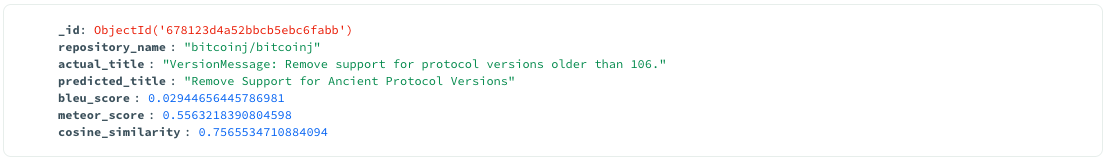
\includegraphics[width=\linewidth]{figures/esempioPredizione.png}
        \caption{saved title generation}     
\end{figure}
\subsubsection{Pull Request Preprocessing}
Pull requests are pre-processed to ensure data integrity and avoid compromising model performance. In particular, an initial filtering is performed during the creation of the training and test sets, in order to exclude pull requests with empty fields. Subsequently, the data is split into training and testing sets using the \texttt{train\_test\_split} function from the \texttt{sklearn} library. Furthermore, the \texttt{diff} field, which is usually very long and rich in information, is manipulated in order to keep only the information useful to the model. For this purpose, the function \texttt{extract\_diff\_details} has been implemented, whose purpose is to extract key information from the \texttt{diff} text. The function, shown below, uses regular expressions to find specific items of interest:

\begin{minted}[bgcolor=gray!5, breaklines=true, fontsize=\small, frame=single, linenos=true]{python}
def extract_diff_details(diff_text):
    comments = re.findall(r'//.*|/\*.*?\*/', diff_text, re.DOTALL)
    class_names = re.findall(r'\bclass\s+(\w+)', diff_text)
    method_names = re.findall(
        r'\b(?:public|private|protected)?\s+[\w<>\[\]]+\s+(\w+)\s*\(.*?\)\s*\{', diff_text
    )
    pom_add_dependencies = re.findall(
        r'<dependency>.*?<artifactId>(.*?)</artifactId>.*?</dependency>', diff_text, re.DOTALL
    )
    pom_remove_dependencies = re.findall(
        r'<!--.*?REMOVE.*?<artifactId>(.*?)</artifactId>.*?-->', diff\_text, re.DOTALL
    )
    return {
        "comments": comments,
        "class_names": class_names,
        "method_names": method_names,
        "added_dependencies": pom_add_dependencies,
        "removed_dependencies": pom_remove_dependencies
    }
\end{minted}
The \texttt{extract\_diff\_details} function works as follows:
\begin{itemize}
\item \textbf{Comments}: Uses the regular expression \texttt{//.*|/\*.*?\*/} to extract both inline and multiline comments in the code.
\item \textbf{Class Names}: Finds all class declarations using the regular expression \texttt{\textbackslash bclass\textbackslash s+(\textbackslash w+)}.
\item \textbf{Method Names}: Recognizes method names by parsing declarations with optional visibility (\texttt{public}, \texttt{private}, \texttt{protected}) and returns the names of the defined methods.
\item \textbf{Added Dependencies in \texttt{pom.xml}}: Finds added dependencies in \texttt{pom.xml} files, by getting \texttt{artifactId} values.
\item \textbf{Removed Dependencies in \texttt{pom.xml}}: Finds removed dependencies marked with comments with the \texttt{REMOVE} tag.
\end{itemize}

This processing allows to reduce the complexity of the \texttt{diff}, keeping only the information useful to the model. The final result is a cleaner, more structured and informative dataset, ideal for training and evaluating the model.
\subsubsection{Contextual Data Retrieval}
A random subset of pull requests is selected from the training set as the context for the LLM using the \texttt{retrieve\_context} function. This only happens in experiments where a \textit{one-shot} or \textit{few-shot} prompt is used to provide context to the model; in other experiments, this function is not used.
The \texttt{retrieve\_context} function selects a random subset of pull requests from the training set, which is used as the context for the LLM. The function takes two parameters: the \texttt{train\_set} which represents the training set and \texttt{n}, which indicates the number of pull requests to extract. For each request, the function randomly selects an element from the set, removes it from the set to avoid duplicates, and adds it to the \texttt{context\_pr} list. This process continues until \texttt{n} pull requests are selected.
\begin{minted}[bgcolor=gray!5, breaklines=true, fontsize=\small, frame=single, linenos=true]{python}
context = retrieve_context(train_set, 3)

def retrieve_context(train_set, n):
    context_pr = []
    while n > 0:
        pr = random.choice(train_set)  % Selects a random pull request from the set
        train_set.remove(pr)           % Removes the selected pull request to avoid duplicates
        context_pr.append(pr)          % Adds the pull request to the context list
        n -= 1                         % Decrements the counter
    return context_pr                 % Returns the context list
\end{minted}
\subsection{LLM Integration}
Once the pull request (PR) preprocessing is completed, the title and body message generation process is started for each PR in the test set. The first step is to remove the "title" and "body message" fields from the pull request data, in order to prepare the model for generation. Next, the generate\_title()/generate\_body\_message() function is called, which is passed the metadata needed to create the new title or body message, along with any context to include if one-shot or few-shot prompts are used.
The function is responsible for structuring the prompt, which varies based on the type of configuration selected (one-shot, few-shot, etc.). If one-shot or few-shot prompts are used, a relevant context is added to the information already present in the dataset to allow the model to generate more relevant answers. The function then calls the Large Language Model (LLM), which, using the prompt, returns the requested results: a new title or body message for the pull request. The LLM is hosted locally and invoked through a REST API.
\subsection{Postprocessing}
The model response is subjected to a syntactic cleaning to not compromise the metrics score.
\begin{minted}[bgcolor=gray!5, breaklines=true, fontsize=\small, frame=single, linenos=true]{python}
def clean_response(response):
    """
    - Rimuove il prefisso 'title:' o 'body:'.
    - Rimuove caratteri di formattazione non.
    - Mantiene solo spazi singoli e rimuove spazi extra..
    """
    if isinstance(response, list):
        # Se la risposta è una lista, applica la pulizia a ogni elemento
        cleaned_list = [clean_response(item) for item in response if isinstance(item, str)]
        return ''.join(cleaned_list)

    if not isinstance(response, str):  # Verifica che l'input sia una stringa
        raise ValueError("Input must be a string or a list of strings")

    # Rimuove il prefisso 'title:' e caratteri non desiderati
    cleaned_response = re.sub(
        r'^\s*title\s*:\s*|[`*#{}]',  # Matcha 'title:' o caratteri non desiderati
        '',
        response,
        flags=re.IGNORECASE
    )
    # Normalizza gli spazi e rimuove quelli extra
    cleaned_response = re.sub(r'\s+', ' ', cleaned_response).strip()

    return cleaned_response
\end{minted}

\subsection{Data rescue}
After the metrics are calculated, a data structure is prepared for saving in the database.

